\documentclass[12pt,a4paper]{ctexart}
\usepackage{geometry}
\geometry{left=2.5cm,right=2.5cm,top=2.5cm,bottom=2.5cm}
\usepackage{listings}
\usepackage{xcolor}
\usepackage{booktabs}
\usepackage{amsmath}
\usepackage{tikz}
\usetikzlibrary{positioning,arrows}
\usepackage{graphicx}
\usepackage{tcolorbox}
\tcbuselibrary{skins,breakable}
\usepackage[colorlinks,linkcolor=blue!70!black,urlcolor=blue!60!black]{hyperref}

\definecolor{themecolor}{RGB}{30,64,175}
\definecolor{codebg}{RGB}{245,247,250}
\definecolor{codeframe}{RGB}{100,116,139}

\usepackage{titlesec}
\titleformat{\section}{\Large\bfseries\color{themecolor}}{\thesection}{0.8em}{}[\vspace{-0.5em}\rule{\textwidth}{0.4pt}]
\titlespacing*{\section}{0pt}{1.2em}{0.6em}
\titleformat{\subsection}{\large\bfseries\color{themecolor!80}}{\thesubsection}{0.8em}{}
\titlespacing*{\subsection}{0pt}{0.8em}{0.3em}

\lstset{
  basicstyle=\small\ttfamily,
  keywordstyle=\color{blue!80!black}\bfseries,
  commentstyle=\color{green!50!black}\itshape,
  stringstyle=\color{red!70!black},
  numbers=left,numberstyle=\tiny\color{gray},
  backgroundcolor=\color{codebg},
  frame=single,rulecolor=\color{codeframe!40},
  breaklines=true,breakatwhitespace=true,
  language=C++,
  aboveskip=0.8em,belowskip=0.6em
}

\newtcolorbox{webox}{colback=blue!5!white,colframe=themecolor,coltitle=white,fonttitle=\bfseries,title=Web前端展示,boxrule=0.5pt,arc=3pt}

\title{\textbf{编译器设计专题实验报告}\\[0.5em]\Large\color{themecolor}实验二：词法分析扫描器实现}
\author{张凌曜 \quad 2234214014 \quad 计算机2306}
\date{}

\begin{document}
\maketitle

\section{实验目的}
用C++写一个词法分析扫描器，支持多种模式：模式1对输入的符号串逐个分类，模式2对一行代码做完整的词法分析，模式3读取源程序文件（.src）做完整的词法分析并输出每行Token和统计信息。另外设计了主文法的DFA词法规则定义文件，让扫描器能处理代码库中任意源程序。

\section{实验原理}
词法分析是编译的第一步，把源代码字符流拆成一个个有意义的单词（Token）。做法就是逐字符扫描，根据首字符类型进不同分支：字母开头走标识符/关键字识别，数字开头走整数或浮点数识别，其他字符处理运算符和界符。

本实验支持的词法类别包括：标识符（ID）、9个关键字（int/float/void/if/else/while/return/input/print）、整数（NUM）、浮点数（FLOAT）、算术运算符（+、-、*、/）、关系运算符（<、>、<=、>=、==、!=）、赋值符=、逻辑运算符（\&\&、$||$）、括号和分号等。

\section{实验过程}

\subsection{识别流程}
扫描器逐字符读入，先跳过空白符，再看首字符：

\begin{center}
\begin{tikzpicture}[node distance=1.2cm,auto,
  box/.style={draw,rounded corners,minimum width=2.8cm,minimum height=0.7cm,fill=blue!8,align=center}]
  \node[box] (start) {开始扫描};
  \node[box,below of=start] (skip) {跳过空白符};
  \node[box,below of=skip] (check) {判断首字符类型};
  \node[box,below left=1.2cm and 1.2cm of check] (alpha) {字母: 标识符};
  \node[box,below of=check] (digit) {数字: 整数/浮点};
  \node[box,below right=1.2cm and 1.2cm of check] (other) {其他: 运算符};
  \path[->,thick] (start) edge (skip) (skip) edge (check)
    (check) edge (alpha) (check) edge (digit) (check) edge (other);
\end{tikzpicture}
\end{center}

\subsection{实现要点}
浮点数判断比较麻烦，得处理三种格式：普通小数（123.45）、小数点开头（.45）、科学计数法（1e-3）。我的做法是先找有没有'e'或'E'，有的话分离基数和指数分别验证；没有的话就数小数点个数，恰好1个就是浮点数。从DFA的角度看，这个过程本质上也是状态转移：读入数字进入“整数”状态，遇到小数点转移到“小数部分”状态，遇到\texttt{e/E}再转移到“指数”状态（指数部分还可能读入正负号），最终停在哪个接受状态就决定是NUM还是FLOAT。

双字符运算符（<=、>=、==、!=、+=、++）必须在单字符之前判断，不然``<=''会被拆成``<''和``=''两个Token。同理，浮点数判断得在整数判断之前，不然``3.14''会被拆成``3''和``.14''。

关键字识别比较简单，先当普通标识符读出来，再查关键字表看是不是关键字就行。关键字表用的是\texttt{std::set<string>}实现，查找复杂度$O(\log n)$，关键字数量少所以效率足够。

\subsection{DFA词法规则文件}
为支持主文法，设计了\texttt{main\_grammar.dfa}文件，用DFA五元组形式定义了每种Token的状态转移规则：标识符/关键字DFA（字母开头，字母或数字继续）、整数DFA（数字序列）、浮点数DFA（含小数点和科学计数法的7个状态）、比较运算符DFA（<、>、=、!的双字符转移）等。共8类Token DFA，覆盖代码库中所有.src文件的词法需求。

另外，扫描器还处理了\texttt{//}行注释：遇到连续两个斜杠就跳过该行剩余内容。

\section{测试结果}

\subsection{模式1测试}
输入：\texttt{5 / id if 485 841.6541 www}

\begin{table}[h]
\centering
\begin{tabular}{cc}
\toprule
输入 & 输出 \\
\midrule
id & ID \\
if & IF \\
485 & NUM \\
841.6541 & FLOAT \\
www & ID \\
\bottomrule
\end{tabular}
\end{table}

\begin{center}

\includegraphics[width=0.9\textwidth]{image/1.png}
\end{center}

\subsection{模式2测试}
输入代码：\texttt{while(true) \{int a=0;\}}

输出：WHILE, LPAR, ID, RPAR, LBR, INT, ID, ASG, NUM, SEMI, RBR

其中\texttt{true}没作为关键字处理（按标识符输出ID），\texttt{int}正确识别为INT。这里\texttt{true}输出ID是符合预期的——本实验定义的关键字集合只包含9个（int/float/void/if/else/while/return/input/print），没有把布尔字面量\texttt{true}纳进去，所以词法分析器把它当作合法标识符处理。

\begin{center}

\includegraphics[width=0.9\textwidth]{image/2.png}
\end{center}

\section{选做：整合DFA}
在词法分析器的基础上加入了菜单系统，程序启动后可以选择四种功能：符号串分类（模式1）、代码行分析（模式2）、源文件扫描（模式3）、DFA字符串识别（模式4）。

模式3可以读取任意\texttt{.src}文件，逐行扫描并输出每个Token的类型、值和行号，最后给出统计摘要。经测试，代码库中33个.src文件均可正确解析。

模式4（DFA整合）的思路：读取\texttt{.dfa}文件加载五元组，用转移表查表做字符串识别，输出状态路径和接受/拒绝结果。

测试：加载\texttt{dfa\_in1.dfa}，输入字符串\texttt{ab}，程序输出路径 $1 \to 2 \to 3$，判定为接受。

\begin{center}
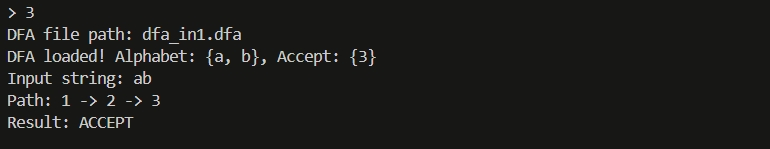
\includegraphics[width=0.9\textwidth]{image/3.png}
\end{center}

\section{实验总结}
这个实验主要踩了两个坑：一个是判断顺序很重要，浮点数必须在整数前面判断，双字符运算符必须在单字符前面判断；另一个是科学计数法的指数部分可能带正负号（1e-3），不能一看到减号就当成减法运算符。

选做部分把DFA整合进来后，可以直观地看到词法分析和DFA模拟的关系——词法分析器内部其实就是多个DFA在并行工作，每个Token类别对应一个DFA。

词法分析器虽然只是编译的第一步，但Token流的质量直接影响后面语法分析，所以边界情况处理还是比较重要的。

\begin{webox}
本实验的词法分析功能已实现为Web前端页面，与C++版scanner逻辑完全一致。

\textbf{主要功能：}源代码输入、逐行Token流展示（彩色标签区分关键字/标识符/数字/运算符/界符）、Token统计信息（总数、各类别计数、标识符与数字列表）。

\begin{center}

\includegraphics[width=0.9\textwidth,height=5.5cm,keepaspectratio]{image/web.png}
\end{center}

前端词法分析器支持全部9个关键字、整数/浮点数（含科学计数法）、双字符和单字符运算符的识别，可处理\texttt{//}行注释。
\end{webox}

\appendix
\section{附录：代码仓库}
本实验的全部源码、报告及Web演示平台已托管至GitHub：

\texttt{https://github.com/yaossss123/compilation-web}

\end{document}
